%% 
%% Technical Paper Template for CCS
%%
%% Adapted from SIGCONF Proceedings template
%%

%%
%% The first command in your LaTeX source must be the \documentclass command.
\documentclass[sigconf, pbalance]{acmart}

\usepackage{tabularx}
\usepackage{array}

%%
%% Inline SQL keywords. Use \sql{...}; it works inside tables and captions.
\definecolor{sqlkeyword}{HTML}{2F5D8C}
\newcommand{\sql}[1]{\texttt{\textcolor{sqlkeyword}{\bfseries #1}}}

%%
%% Let long \texttt identifiers break after underscores, and give TeX some
%% slack before it overfills a line.
\AtBeginDocument{%
  \let\oldunderscore\_%
  \renewcommand{\_}{\oldunderscore\allowbreak}}
\setlength{\emergencystretch}{1.5em}

\AtBeginDocument{%
  \providecommand\BibTeX{{%
    \normalfont B\kern-0.5em{\scshape i\kern-0.25em b}\kern-0.8em\TeX}}}

%%
%% Remove the ACM References statement and copyright notice.
\settopmatter{printacmref=false}
\renewcommand\footnotetextcopyrightpermission[1]{}


%%
%% Majority of ACM publications use numbered citations and references.
%% For managing citations, it is recommended to use bibliography files in BibTeX format.
%% You can then either use BibTeX with the ACM-Reference-Format style,
%% or BibLaTeX with the acmnumeric or acmauthoryear sytles, that include
%% support for advanced citation of software artefact from the
%% biblatex-software package, also separately available on CTAN.
%%
%% Look at the sample-reference.bib file enumerating your References.


%% %% %% %% %%
%% Start of the actual paper.
\begin{document}

%%
%% Paper title.
\title{Rymming Stroking and Sucking}

%%
%% Authors
\author{Jack Clavano}
\affiliation{%
  \institution{De La Salle University}
  \city{Manila}
  \country{Philippines}}
\email{angelica\_therese\_clavano@dlsu.edu.ph}

\author{Enrique Miguel Aragon}
\affiliation{%
  \institution{De La Salle University}
  \city{Manila}
  \country{Philippines}}
\email{enrique\_aragon@dlsu.edu.ph}

\author{Jacoba Ysabelle Luna}
\affiliation{%
  \institution{De La Salle University}
  \city{Manila}
  \country{Philippines}}
\email{jacoba\_luna@dlsu.edu.ph}

\author{Zhean Robby Ganituen}
\affiliation{%
  \institution{De La Salle University}
  \city{Manila}
  \country{Philippines}}
\email{zhean\_robby\_ganituen@dlsu.edu.ph}


%%
%% By default, the full list of authors will be used in the page headers.
%% Often, this list is too long and will overlap other information printed in the page headers. 
%% This command allows the author to define a more concise list of authors' names for this purpose.
\renewcommand{\shortauthors}{Trovato et al.}


%%
%% The abstract is a short summary of the work to be presented in the article.
\begin{abstract}
This set of guidelines for formatting your research paper has been adapted from the formatting guidelines for ACM SIG Proceedings. The Abstract should consist of 150 to 250 words in a single paragraph that provides the reader with a summary of your research/project and what you intend to do. It gives a brief description of the motivation for your research/project, the problem you intend to cover, the purpose and method for conducting your study, and your results and findings.
\end{abstract}


%%
%% Keywords
%% The author(s) should pick words that accurately describe the work being presented. 
%% Separate the keywords with commas.
%% Aside from proper nouns and acronyms, only the first letter of the first keyword should be capitalized
\keywords{Data Warehouse, ETL, OLAP, Query Processing, Query Optimization}

%%
%% This command processes the author and affiliation and title information and builds the first part of the formatted document.
\maketitle

\section{Introduction}
\label{sec:introduction}

The Dutch railway network is very highly utilized compared to those of other countries. NS and several other operators run their trains on the same infrastructure, and the time buffers between trains are what keep a delay on one train from spreading to the next \cite{kroon2008dutch}. Measuring punctuality, cancellations, and station congestion for a whole year therefore means working with tens of millions of stop events. Records at this volume are hard to analyze in their raw form and need a structure built for aggregation.

This paper describes how we turned one year of raw Dutch railway records into a dimensional data warehouse in PostgreSQL and built an OLAP application on top of it. This section defines the railway terms used in the paper, describes the dataset, summarizes the exploratory data analysis (EDA) that shaped the design, and states who the warehouse is for.

The code is available at \url{https://github.com/zrygan/mono4db}, with the warehouse and ETL pipeline in \texttt{dutch\_railway/} and the OLAP application in \texttt{dutch\_railway-app/}.

\subsection{Definition of Terms}
\label{subsec:definitions}

\begin{itemize}
    \item \textbf{Service.} One scheduled train trip from its origin to its terminus, identified in the dataset by \texttt{Service:RDT-ID}.
    \item \textbf{Stop.} One call of a service at one station, identified by \texttt{Stop:RDT-ID}. A stop has an arrival, a departure, or both. A service is made up of one or more stops, and this two-level structure gives the warehouse its two fact tables.
    \item \textbf{RDT.} Short for \emph{Rijden de Treinen} (``Are the trains running''), the Dutch service that collects the real-time departure data published by the national operator NS and keeps the archive this dataset comes from \cite{rijdendetreinen, szarnyas2024railway}. The prefix in the identifier names refers to this source.
    \item \textbf{Delay.} The difference in whole minutes between the scheduled and the actual time of an arrival or a departure. Trains that run early are recorded with a delay of 0. The dataset records only the delay that was observed and does not give its cause.
    \item \textbf{Punctuality.} The share of trains that arrive within a fixed delay threshold. The Dutch definition counts trains that arrive at one of the 35 main stations with a delay of less than three minutes \cite{kroon2008dutch}.
    \item \textbf{Cancellation.} A service is \emph{completely cancelled} when none of its stops were served and \emph{partly cancelled} when only some were. At the stop level, the arrival, the departure, or both can be cancelled.
    \item \textbf{Train number change.} A service whose train number changes partway through the trip, for example when a train continues past a hub under a new number.
    \item \textbf{Replacement service.} A bus, metro, or taxi that runs in place of a train, usually during engineering works. In the dataset these have service types ending in \emph{ipv trein} (``instead of train'').
\end{itemize}

\subsection{Dataset Description}
\label{subsec:dataset}

The dataset covers every service on the Dutch network in the 2025 calendar year. It contains $22{,}226{,}311$ rows. Each row is one stop of one service. The rows cover $2{,}402{,}665$ services over 365 days and 578 station codes, a count that includes stations outside the Netherlands served by international trains.

Each row has 20 columns that fall into two groups. The \texttt{Service:*} columns describe the whole trip and repeat on every stop of it. These are the service identifier, date, type (e.g., ``Intercity'' or ``Sprinter''), operating company, train number, the two cancellation flags, and the maximum delay of the trip. The \texttt{Stop:*} columns describe one stop. These are the stop identifier, the station code and name, the arrival and departure times with their delays and cancellation flags, the planned and actual platform, and a platform change flag.

\subsection{Exploratory Data Analysis}
\label{subsec:eda}

To help inform the data warehousing stage, we first profiled the entire database via EDA.

\begin{table}[t]
\centering
\small
\caption{Null values by column group}
\Description{Distribution of missing values across raw attribute groups, showing counts, percentages, and root causes.}
\label{tab:eda_columns}
\begin{tabularx}{\columnwidth}{l r r X}
\toprule
\textbf{Column group} & \textbf{Null rows} & \textbf{Null \%} & \textbf{Cause} \\
\midrule
Other 12 columns & 0 & 0.0\% & None \\
Arrival (3 columns) & $2{,}403{,}837$ & 10.8\% & Trip origin \\
Departure (3 columns) & $2{,}404{,}493$ & 10.8\% & Trip terminus \\
Platform (2 columns) & $3{,}008{,}309$ & 13.5\% & Mixed \\
\bottomrule
\end{tabularx}
\end{table}

\subsubsection{Null values}
Only 8 of the 20 columns contain nulls, and they fall into three groups (Table~\ref{tab:eda_columns}). Within each group the columns are always null together. The arrival group holds the arrival time, delay, and cancellation flag. When the stops of each service are ordered by time, 99.9\% of the null arrivals fall on the first stop, which is the origin of the trip and has no arrival. In the same way, 99.9\% of the null departures fall on the last stop. These nulls are therefore part of the structure of a trip and not missing data.

Replacement buses and metros never have a platform because they do not stop at a track, and cancelled stops never have one because no track was assigned. However, foreign operators such as DB and NMBS, leave the platform empty for 60\% to 93\% of their served stops, while Dutch operators leave it empty for less than 3\%. 

\subsubsection{Delays of cancelled stops}
Every cancelled arrival and every cancelled departure has a delay of 0 minutes, which affects about 1.1 million rows. Averaging these values would make cancelled trains count as on time. But replacement buses and metros never report a delay above 0 for the whole year, this likely means that no real-time tracking was available.

\subsubsection{Cancellation flags}
The two service-level flags overlap instead of excluding each other. Of the $52{,}098$ services flagged as completely cancelled, $50{,}262$ are also flagged as partly cancelled. The remaining $1{,}836$ have no cancelled stops at all, even though the whole service is marked as cancelled. The stop-level flags are therefore a more reliable record of which stops were actually served.

\subsubsection{Codes that change during the year}
The yearly timetable change on 14 December 2025 changed several identifiers. Operator names were cut to 10 characters (for example \texttt{DB} became \texttt{Deutsche B}), and between 14 and 18 December some services carried numeric operator codes instead of names. Berlin Hauptbahnhof appears as \texttt{BERHBL} for the whole year and also as \texttt{BERHBT} from 14 December onward. The code \texttt{LAND} is the only code with two station name, it was used for Landeck-Zams in early February and for Venezia Santa Lucia from mid February.

\subsubsection{Stops after midnight}
Each service has one \texttt{Service:Date}, but services that run late in the evening have stops on the following day. In 2025, $745{,}493$ arrivals fall on a later calendar date than their service, and $11{,}503$ stops arrive before midnight and depart after it. Taking the date of a stop from its service would place these stops before the start of the trip.

\subsubsection{Train numbers}
A service can change its train number along the route. This happens in $12{,}568$ services, never more than once per service. The same train number can also belong to several operators and service types during the year. This simply means that train numbers cannot be used as keys.

\subsection{Intended Use and Users}
\label{subsec:usage_users}

The warehouse is designed for three kinds of analysis. The first is comparing operators on punctuality and cancellations. The second is comparing delays across the three time-of-day periods and across months. The third is following a delay from stop to stop within a service to find stations where trains tend to lose time and stations where they make it up.

These analyses serve four groups of users.
\begin{enumerate}
    \item \textbf{Infrastructure planners}, who need to know which stations and periods have the most delay when they plan timetables.
    \item \textbf{Train operating companies}, who need to track the punctuality and cancellations of their own services.
    \item \textbf{Transport authorities}, who need to check whether operators meet the punctuality terms of their concessions.
    \item \textbf{Data engineers}, who can use the warehouse as a test case for loading and querying a large analytical dataset.
\end{enumerate}

\section{Data Warehouse}\label{sec:data_warehouse}

\begin{figure*}[t]
\centering
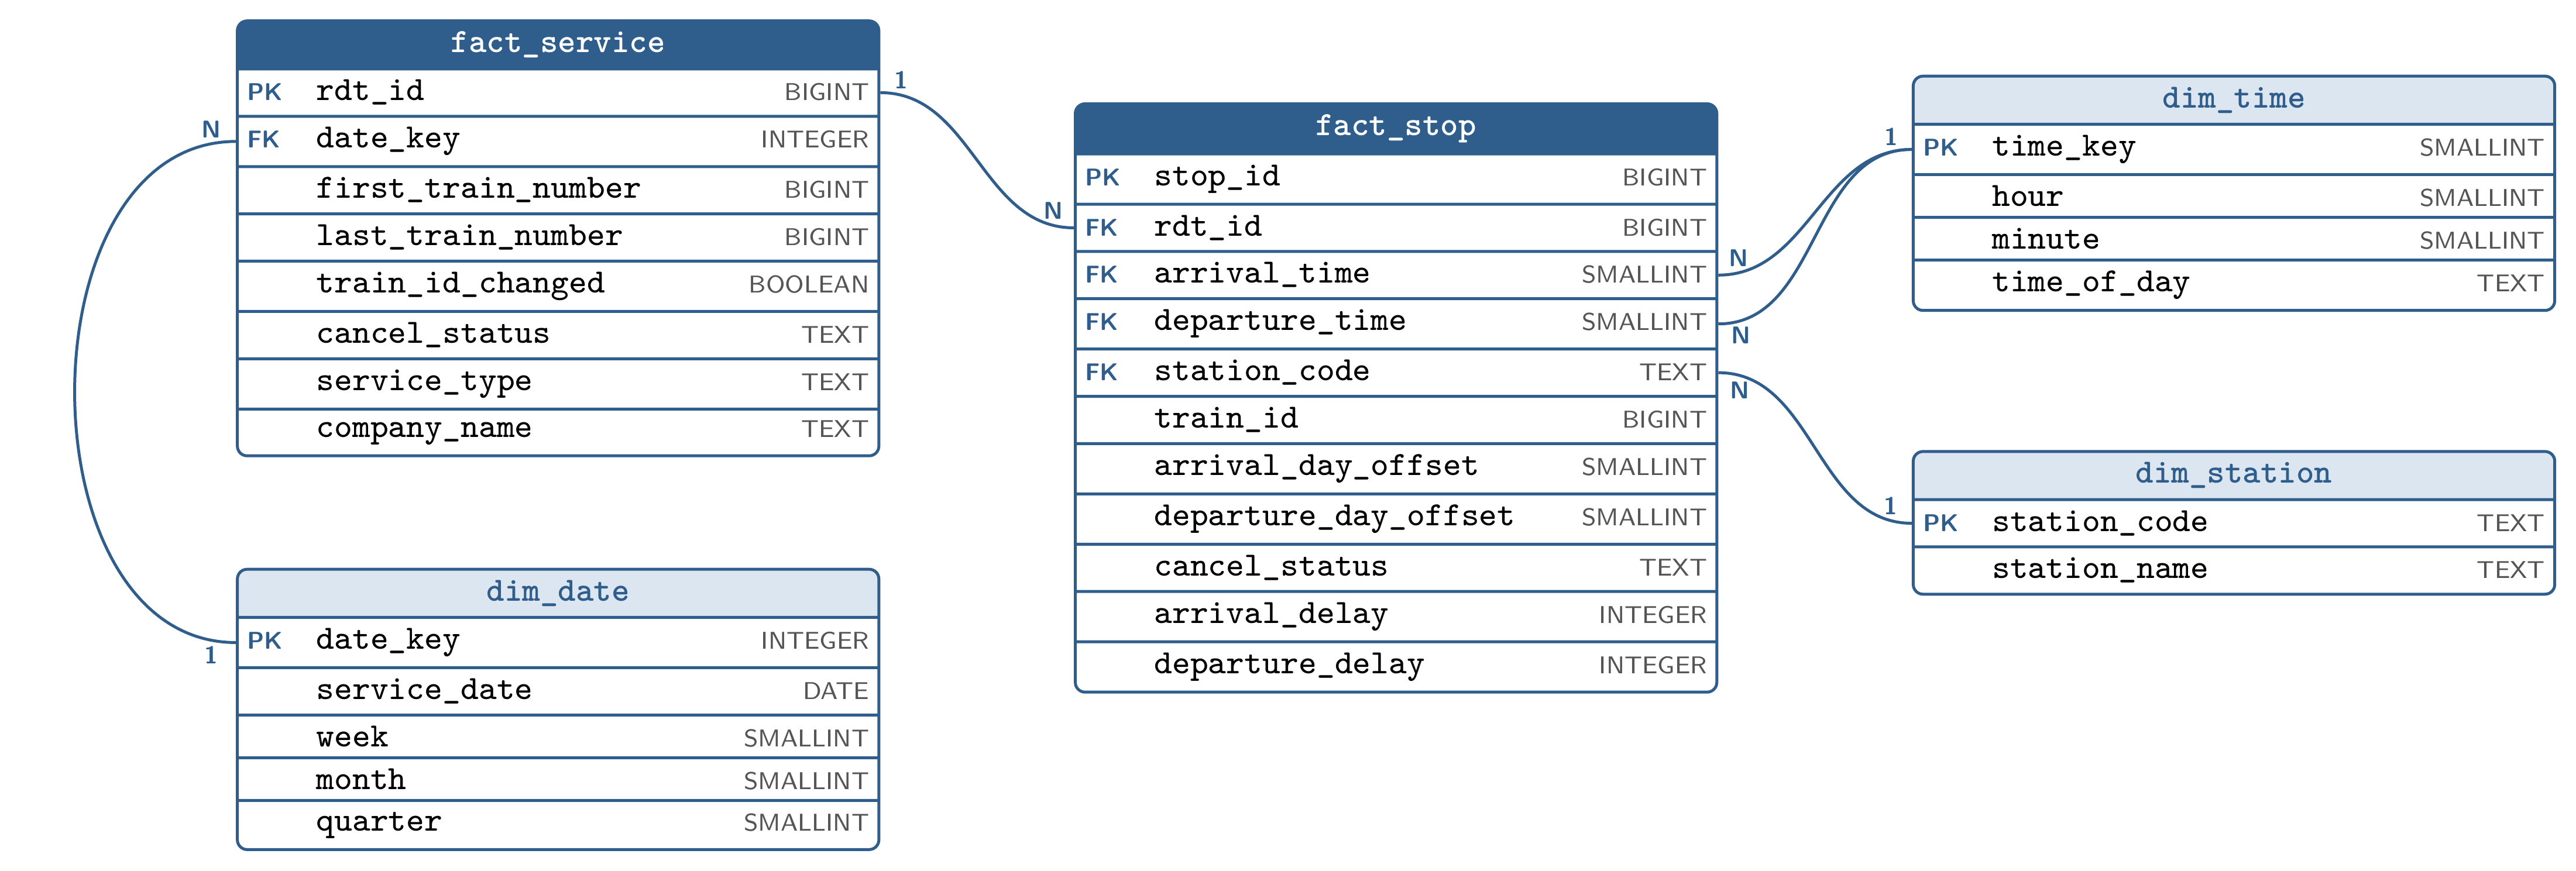
\includegraphics[width=\textwidth]{figures/schema.png}
\caption{Schema of the data warehouse. Dark headers are fact tables and light headers are dimension tables. Each line joins a foreign key (N) to the primary key it references (1).}
\Description{Entity-relationship diagram of the warehouse. fact\_service references dim\_date through date\_key. fact\_stop references fact\_service through rdt\_id, dim\_time through arrival\_time and departure\_time, and dim\_station through station\_code.}
\label{fig:schema}
\end{figure*}

The creation of the database schema seen in Figure~\ref{fig:schema} was informed by the aforementioned EDA and domain knowledge. Given that the schema utilizes 2 fact tables, 
\textit{fact\_service} and \textit{fact\_stop}, it is a galaxy schema by definition \cite{g4g-galaxy}, though it retains the principles of a star schema design as well. The decision 
to use two fact tables was driven the difference in granularity between the two tables, as the service table corresponds to a train's entire trip, while the stop 
table represents one arrival or departure within a trip. 

The service table contains an RDT ID as its primary key, along with a date key as its foreign key. The service table also contains fields that denote 
whether or not its train changed midway, whether the service was cancelled (and to what degree), its service type, and the name of the company administering the service.
The stop table contains a stop ID as its primary key, while its foreign keys consist of the RDT id of its corresponding service, the arrival and derparture times, and
the station code. Additionally, it contains information regarding train ID, arrival and departure day offset, cancellation status, and arrival and departure delays. The two
fact tables are connected by a one-to-many relationship from the stop table to the service table, as one train service contains multiple stops itself.

To provide further context to the existing fact tables, three dimensional tables were created, \textit{dim\_time}, \textit{dim\_station}, and \textit{dim\_date}. 
The time and station dimensions connect to the stop table, while the date dimension connects to the service table. The time dimension's hierarchy focuses on drilling down 
from a general time of day (morning, afternoon, evening) to the hour, and then by the minute. It has two instances of a one-to-many relationship with the stop table, as the 
2 relationships pertain to the arrival and departure times to and from a stop. The station dimension contains the station's code and its name, and maintains a one-to-many 
relationship with the stop table as well since one station houses multiple instances of a train stopping there. Lastly, the date dimension connects to the service table, and its 
hierarchy focuses on drilling down from the quarter, to month, to week, and then to the service's actual date. Similar to the other dimension tables, it has a one-to-many 
relationship with its corresponding fact table, as every day sees multiple train services.

One of the challenges that we encountered in the creation of the data warehouse was the initial difficulty in understanding the relationships between the columns. It took 
a collective effort backed by domain research on the Dutch railway system to break down the meaning of terms such as \textit{service}, \textit{stop}, \textit{RDT}, and 
\textit{cancellation} within the context of the dataset. Another challenge initially faced concerned the size of the dataset, which made it difficult and extremely time-consuming 
to open. In order to circumvent this, \textit{OpenRefine} was used to initially view the data, which was then codensed into an Apache Parquet file that significantly reduced its size. 
Afterwards, the data became more manageable to handle, especially for tasks such as the EDA performed earlier that provided further insight into the dataset that would inform our
decision-making. It is also worth noting that the original CSV file of the dataset contained 3 columns named \textit{Stop: Platform change}, \textit{Stop: Planned 
platform}, and \textit{Stop: Arrival platform}  that focus on the platform where a train stopped. However, this is not as much of a measure of efficiency compared to time, 
station, and date. Additionally, these 3 columns are not listed in the DuckDB documentation's list of columnns in the dataset, so they were ommitted 
from the creation of the database schema. 

\section{Extract-Transform-Load (ETL) Script}
\label{sec:etl_script}

The ETL pipeline takes the raw 2025 file from its source, converts it into the tables of the warehouse, and loads them into PostgreSQL 17. It is implemented in Python using Apache Airflow.

\subsection{Design Constraints}
\label{subsec:etl_constraints}

The following constraints are considered in the implementation of the ETL pipeline:
\begin{enumerate}
    \item Because the uncompressed CSV file is 3.37\,GB and risks exhausting available RAM under full ingestion, we delegate all parsing and transformation to DuckDB \cite{raasveldt2019duckdb}. DuckDB processes the input out-of-core in a streaming pipeline, constrained to a 2\,GB memory limit and 4 execution threads.
    \item Row-by-row \sql{INSERT} statements are slow at this volume. Each inserted row updates every index on the table and is checked against every foreign key. The PostgreSQL documentation recommends loading large tables with \sql{COPY}, creating indexes after the data is in, and dropping foreign key constraints during the load \cite{postgresql2025populating}.
\end{enumerate}

\subsection{Pipeline Architecture}
\label{subsec:etl_architecture}

\begin{figure}[t]
\centering
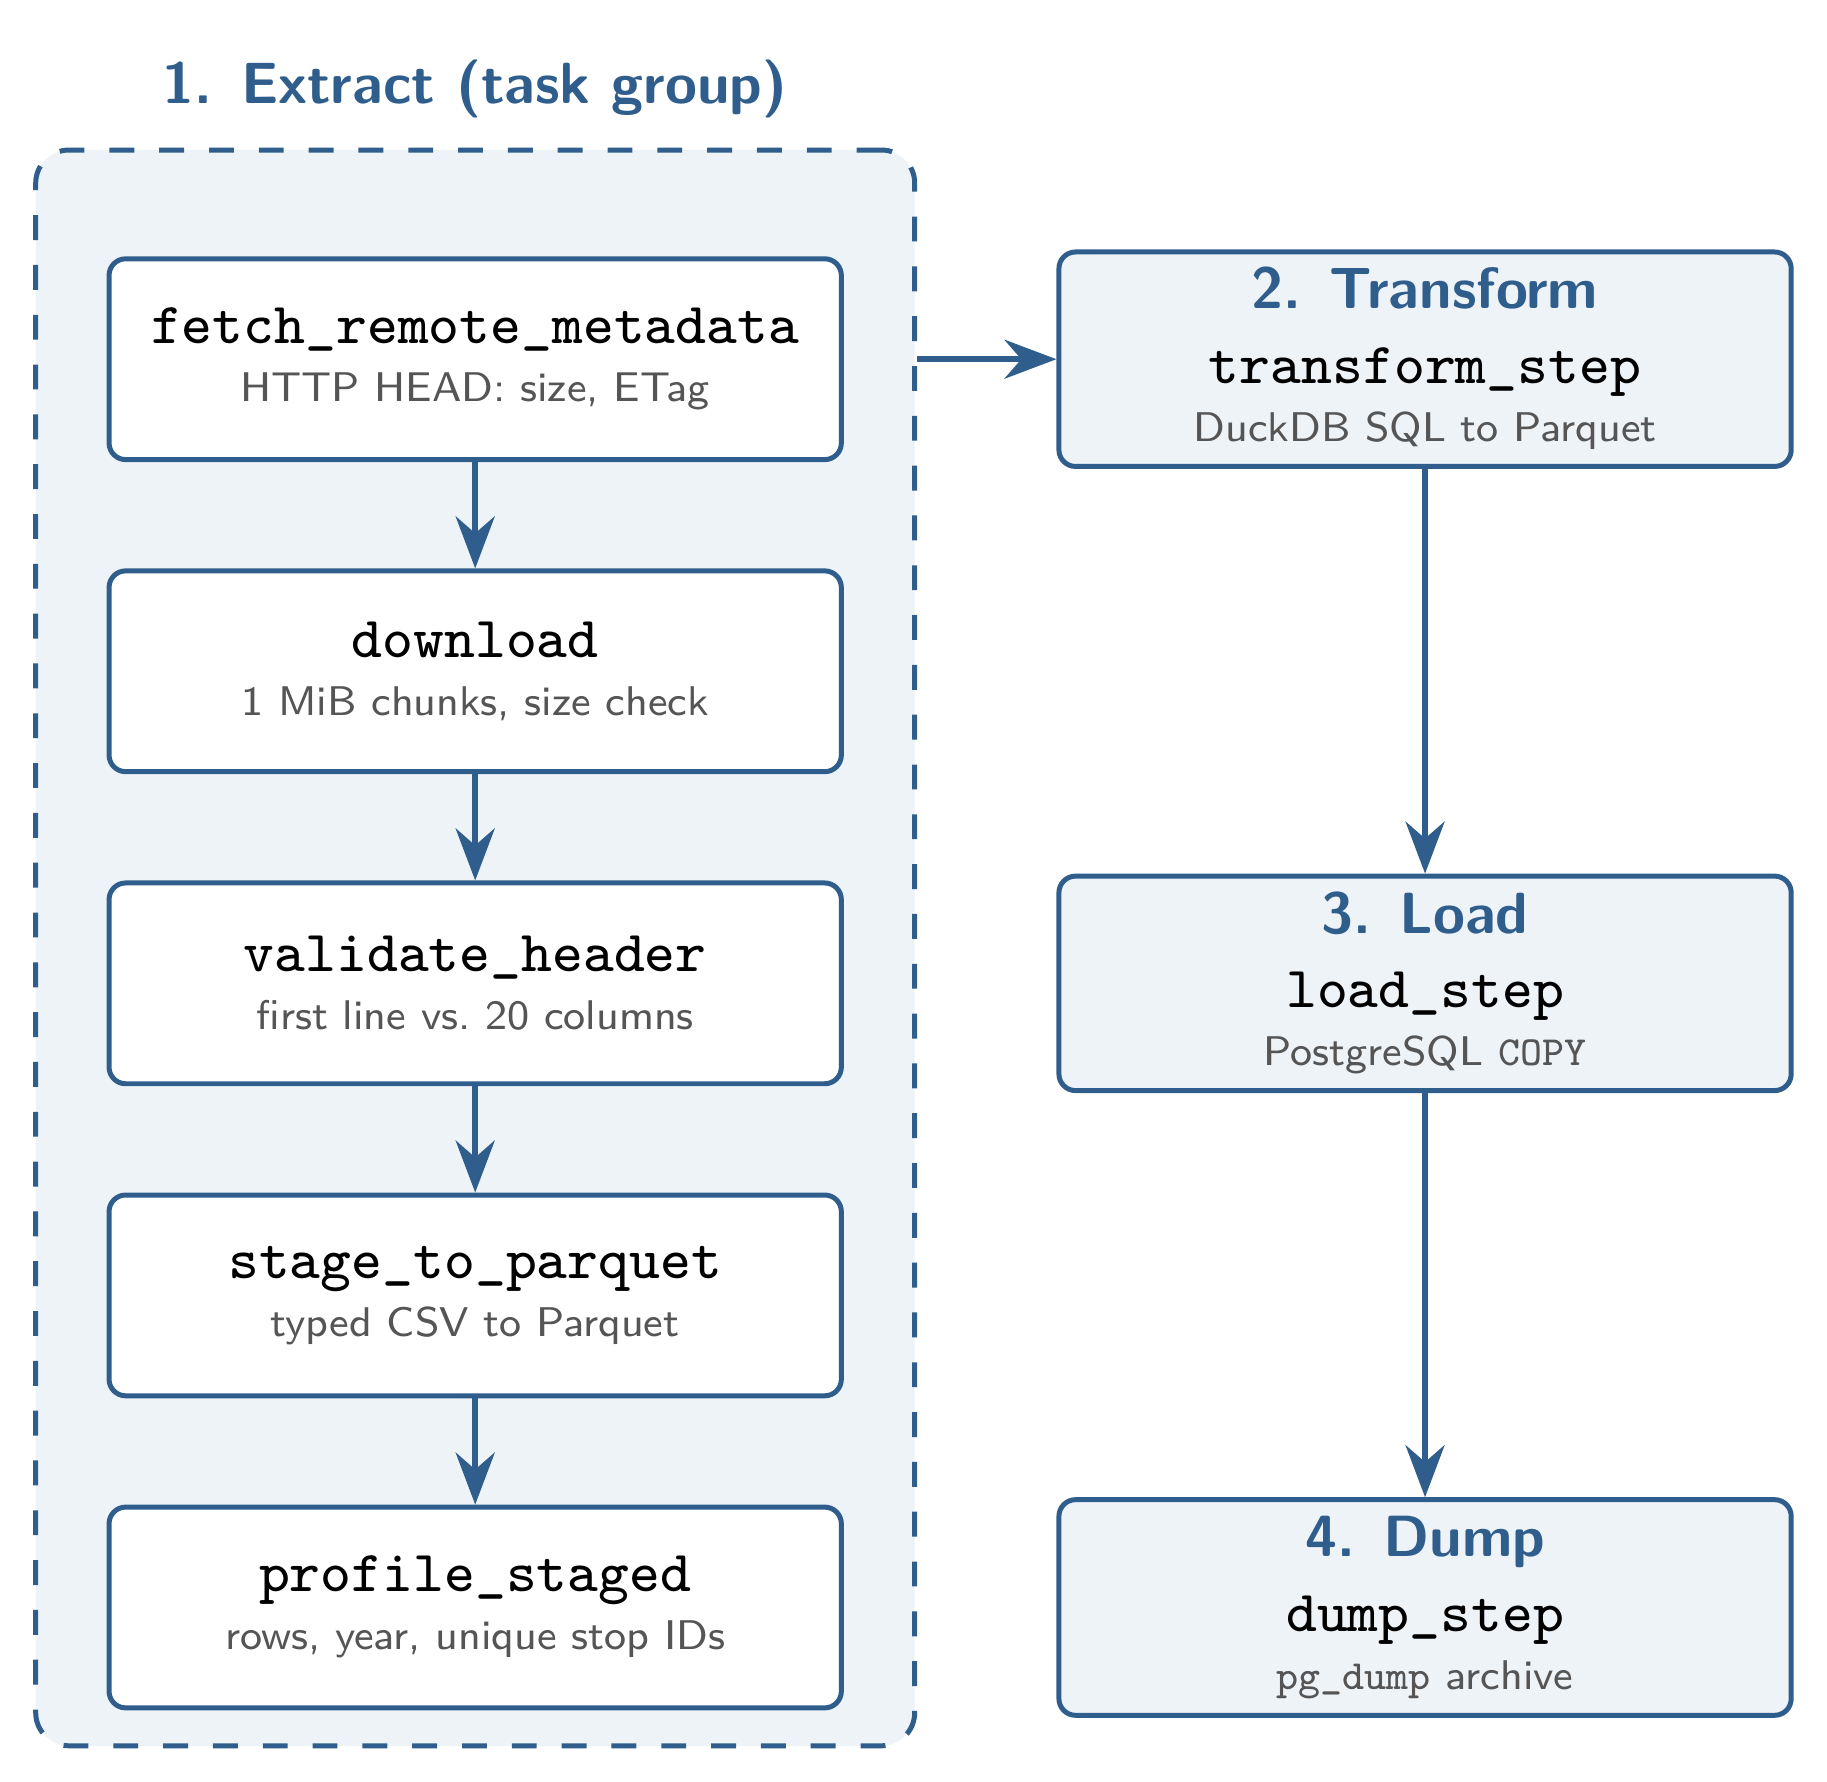
\includegraphics[width=\columnwidth]{figures/etl_dag.png}
\caption{Tasks of the \texttt{dutch\_railway\_etl} Airflow DAG.}
\Description{The Airflow DAG runs an extract task group of five tasks, then a transform task, a load task, and a dump task, in sequence.}
\label{fig:etl_dag_flow}
\end{figure}

The DAG \texttt{dutch\_railway\_etl} runs four stages in sequence (Figure~\ref{fig:etl_dag_flow}). Each task retries twice before failing. Every file the pipeline writes is first written under a temporary \texttt{.part} name and then renamed, so a failed task never leaves a half-written file in place of a complete one.

\subsubsection{Extract}
\label{subsubsec:extraction}

\texttt{fetch\_remote\_metadata} sends an HTTP \texttt{HEAD} request to the source and reads the file size and \texttt{ETag}. \texttt{download} skips the download when a local copy exists whose size and \texttt{ETag} match the values saved in a sidecar file from the previous run. Otherwise it streams the file to disk in 1\,MiB chunks and checks the number of bytes received against the reported size before renaming the file. \texttt{validate\_header} reads only the first line of the compressed file and checks that the column names and their order match the expected 20 columns.

\texttt{stage\_to\_parquet} then has DuckDB read the CSV with an explicit type for every column instead of letting it guess types, and writes it to a Zstandard-compressed Parquet file. The session time zone is set to \texttt{Europe/Amsterdam} so that all timestamps are read in Dutch local time. Finally, \texttt{profile\_staged} checks that the staged file is not empty, that every service date falls in the requested year, and that \texttt{Stop:RDT-ID} is unique.

\subsubsection{Transform}
\label{subsubsec:transformation}

The transform stage defines a DuckDB view over the staged file and runs one SQL query per warehouse table. The view applies the station code corrections and adds a sort key for the stops of a service, ordered by time and then by stop identifier. Each query writes its result to its own Parquet file. \texttt{dim\_date} is generated with one row per day between the first and the last service date. \texttt{dim\_time} is generated with one row for each of the 1,440 minutes of a day. \texttt{dim\_station}, \texttt{fact\_service}, and \texttt{fact\_stop} are derived from the staged rows. Table~\ref{tab:transformation_rules} lists the rules applied to individual columns.

\begin{table*}[t]
\centering
\small
\caption{Transformation rules}
\Description{Rules applied to individual warehouse columns during the transform stage, with the reason for each.}
\label{tab:transformation_rules}
\begin{tabular}{>{\raggedright\arraybackslash}p{0.27\textwidth} >{\raggedright\arraybackslash}p{0.68\textwidth}}
\toprule
\textbf{Column} & \textbf{Rule} \\
\midrule
\texttt{dim\_station.station\_code} &
\texttt{LAND} with the name Venezia Santa Lucia becomes \texttt{VENEZ}, and \texttt{BERHBT} becomes \texttt{BERHBL}. Each code then names exactly one station, and Berlin Hbf has one code. \\
\addlinespace
\texttt{dim\_date.date\_key} &
The date as an integer of the form YYYYMMDD, for example 20250312. A year can be selected with a range on the key without joining \texttt{dim\_date}. \\
\addlinespace
\texttt{dim\_time.time\_key}, \texttt{fact\_stop.arrival\_time}, \texttt{fact\_stop.departure\_time} &
The time as an integer of the form HHMM, for example 1430 for 14:30. Seconds are dropped, which affects the 4,961 stops whose times are not on a whole minute. \\
\addlinespace
\texttt{dim\_time.time\_of\_day} &
\texttt{morning} from 05:00 to 11:59, \texttt{afternoon} from 12:00 to 17:59, and \texttt{night} from 18:00 to 04:59. \\
\addlinespace
\texttt{fact\_service.cancel\_status} &
\texttt{completely} if the completely cancelled flag is set, otherwise \texttt{partially} if the partly cancelled flag is set, otherwise \texttt{none}. The completely cancelled flag is checked first because it is usually set together with the other one. \\
\addlinespace
\texttt{fact\_service.first\_train\_number}, \texttt{last\_train\_number}, \texttt{train\_id\_changed} &
The train number at the first and at the last stop of the service, and whether the service has more than one train number. \\
\addlinespace
\texttt{fact\_stop.cancel\_status} &
\texttt{completely} if both the arrival and the departure are cancelled, \texttt{arrival-only} or \texttt{departure-only} if one of them is, and \texttt{none} otherwise. A missing arrival at the origin or a missing departure at the terminus counts as cancelled, so a cancelled origin or terminus is \texttt{completely} cancelled. \\
\addlinespace
\texttt{fact\_stop.arrival\_delay}, \texttt{fact\_stop.departure\_delay} &
\sql{NULL} when the arrival or departure is cancelled, and the source delay otherwise. Averages then only include stops that were served. \\
\addlinespace
\texttt{fact\_stop.arrival\_day\_offset}, \texttt{fact\_stop.departure\_day\_offset} &
The number of days between the service date and the arrival or departure, so that stops after midnight keep their correct order. \\
\bottomrule
\end{tabular}
\end{table*}


After writing the tables, the transform stage checks them before anything is loaded. It verifies that \texttt{fact\_stop} has as many rows as the staged file, that no station code has more than one name, and that every foreign key value in the fact tables exists in the table it refers to.

\subsubsection{Load}
\label{subsubsec:loading}

The load stage puts the transformed tables into the PostgreSQL warehouse. It runs as a single transaction, so a run that fails leaves no partly loaded tables behind.

The loader creates the warehouse tables from \texttt{schema.sql}, including their indexes and foreign keys, and copies the rows of each table into PostgreSQL with \sql{COPY}. The dimensions are loaded first, then \texttt{fact\_service}, then \texttt{fact\_stop}.

To make the copy of 22 million stops faster, the loader removes the indexes and foreign keys of the fact tables before the copy and restores them afterwards. PostgreSQL then builds each index and checks each foreign key once over the whole table instead of once per row, as the PostgreSQL documentation recommends for bulk loads \cite{postgresql2025populating}. The finished tables have all the indexes and constraints defined in \texttt{schema.sql}.

\subsubsection{Dump}
\label{subsubsec:dump}

The last stage writes the five warehouse tables to a \texttt{pg\_dump} archive in custom format.

\subsection{Schema Constraints}
\label{subsec:schema_constraints}

The warehouse enforces the following constraints.
\begin{itemize}
    \item \textbf{Primary keys} on \texttt{date\_key}, \texttt{time\_key}, \texttt{station\_code}, \texttt{rdt\_id}, and \texttt{stop\_id}.
    \item \textbf{Foreign keys} from \texttt{fact\_service} to \texttt{dim\_date}, and from \texttt{fact\_stop} to \texttt{fact\_service}, \texttt{dim\_station}, and \texttt{dim\_time}. \texttt{fact\_stop} refers to \texttt{dim\_time} twice, once for the arrival and once for the departure. Both of these columns allow \sql{NULL} for the origin and the terminus.
    \item \textbf{Check constraints} that limit \texttt{time\_of\_day} and the two \texttt{cancel\_status} columns to the values listed in Table~\ref{tab:transformation_rules}.
    \item \textbf{Secondary indexes} on the foreign key columns used in joins, which are \texttt{fact\_service(date\_key)}, \texttt{fact\_stop(rdt\_id)}, and \texttt{fact\_stop(station\_code)}.
\end{itemize}

\subsection{Issues and Solutions}
\label{subsec:etl_issues}

Table~\ref{tab:etl_issues} lists the problems we had to handle while building the pipeline and how each one was solved.

\begin{table*}[t]
\centering
\small
\caption{Issues handled by the ETL pipeline}
\Description{Summary of data engineering challenges, symptoms, and mitigations implemented in the ETL pipeline.}
\label{tab:etl_issues}
\begin{tabularx}{\textwidth}{l X X}
\toprule
\textbf{Issue} & \textbf{Problem} & \textbf{Solution} \\
\midrule
\textbf{Load speed} &
Inserting 22.2 million rows into tables with indexes and foreign keys updates every index and checks every key for each row. &
Drop the fact table foreign keys and secondary indexes, load with \sql{COPY}, and rebuild them once after the load \cite{postgresql2025populating}. \\
\addlinespace

\textbf{Memory} &
The decompressed file is 3.37\,GB, too large to read into Python memory. &
Read and transform the file in DuckDB with a 2\,GB memory limit, and keep only Parquet files between stages \cite{raasveldt2019duckdb}. \\
\addlinespace

\textbf{Incomplete downloads} &
A dropped connection can leave a truncated file that looks like a valid download. &
Download to a \texttt{.part} file, compare its size with \texttt{Content-Length}, and rename it only if the sizes match. \\
\addlinespace

\textbf{Station codes} &
\texttt{LAND} has two station names, and Berlin Hbf has two codes. &
Remap Venezia Santa Lucia to \texttt{VENEZ} and merge \texttt{BERHBT} into \texttt{BERHBL} during the transform. \\
\addlinespace

\textbf{Delays of cancelled stops} &
About 1.1 million cancelled arrivals and departures have a delay of 0, which would count them as on time. &
Store these delays as \sql{NULL}. \\
\addlinespace

\textbf{Stops after midnight} &
Stops after midnight would get the date of their service, which is the previous day. &
Store an arrival and a departure day offset relative to the service date in \texttt{fact\_stop}. \\
\bottomrule
\end{tabularx}
\end{table*}

\section{OLAP Application}
\label{sec:olap_application}

To make an OLAP application that provides use to society, we focused our application on the reliability of the different entities involved in the Dutch railway system. After a look at the database, the best metric provided to measure reliability is the delay of the train to its stop on arrival and on departure.





\subsection{Dice Observed in All Reports}
\label{subsec:all_dice}
Before generating the report, the user is able to filter out and exclude certain companies, and can further restrict the data to the past 12 months (the full dataset) or the past 6 months. These filters select a subset of members along the dimensions for company and date, and applying them together restricts the two dimensions at once. This is a dice operation, and applies to every report below.





\subsection{Report 1: On-Time Trends}
\label{subsubsec:on-time_trends}
The first report shows the on-time rate of all selected companies per quarter, month, and week.

In the application, there is a bar graph showcasing the difference in on-time rate. Upon initial load, the bar graph shows the data in relation to each quarter of the year. Once the user clicks on it, it shows the data in relation to each month of the year, and then the user can select a month to view the data in relation to the 4 weeks of that month.

\textbf[Picture of the website]

The corresponding SQL query used in this report is as follows:

\textbf[SQL Query here]

The OLAP operation used in this query is drill-down and rollup. Rollup is the process of starting at the smallest grain, then aggregating onto an increasingly larger grain. In this query, the smallest grain is the data per-week. After the per-week data, it gets aggregated to per-month, then per-quarter. Drill-down is a very similar process, but starts from the larger grain down to the smaller grain. In the query, the ROLLUP construct was used, formatting the resulting table in a manner that shows information in the three different grains. Below is a sample of the resulting table from this query:

\textbf[Sample Table]

This report lets users see whether reliability is improving or worsening over time.




\subsection{Report 2: Company Monthly Rank by On-Time Rate}
\label{subsubsec:company_monthly_rank_otr}
The second report details the on-time rate of each selected companies, including each company's rank based on their on-time rate, per month, on a chosen time of day.

In the application, the user is able to pick which time-of-day to filter the data on. There is a line graph, showing the months on the x-axis and the included companies on the y-axis. A line represents a company, and hovering over it highlights that company.

\textbf[Picture of the website]

The corresponding SQL query used in this report is as follows:

\textbf[SQL Query here]

As the performance of the railway system differs at the different times of day, restricting it to show only services from the morning, afternoon, or night allows a more specific analysis of how companies operate at different times. The explicit rankings make it easier as well to identify which companies perform best at different times, and whether the best-performing company changes depending on the time.

The OLAP operation used is slice. The time-of-day dimension is fixed on a single value dependent on user input, and removes all data corresponding to times that are not within the selected time by the user. Below is a sample of the resulting table from this query:

\textbf[Sample Table]

This report shows which companies are most reliable at different times of the day.





\subsection{Report 3: Underperforming Trains in Companies}
\label{subsubsec:underperforming_trains}
The third report focuses on the performance of trains under a specific company. The average arrival delay of a company throughout all of its stops is recorded. The average arrival delay per-train, and the difference of the company average and train average is calculated to see which trains perform worst in each company, relative to the company average.

In the application, the user can pick a company and a number $n$. The average company arrival delay is displayed, alongside a bar graph of the $n$ worst performing trains.

\textbf[Picture of the website]

The corresponding SQL query used in this report is as follows:

\textbf[SQL Query here]

In this query, the company name, train ID, average company delay, average train delay, train on-time delay, and the gap of the train from the company's average delay. Unlike the first two reports, this report focuses on analyzing the performance of trains, which helps identify problematic trains.

The operation used in this query is once again, a slice operation. In this report, rather than altering the time dimension, the slice is performed on the company dimension. All data not operated by the chosen company is removed. Below is a sample of the resulting table from this query:

\textbf[Sample Table]

This report helps a company decide which trains are problematic and may need inspection.





\subsection{Report 4: Station Delay Recovery and Addition}
\label{subsubsec:station_delay_recovery}
The last report focuses on whether a station is able to recover from delays, or make delays worse. In the data warehouse, arrival delay and departure delay are both metrics included per-stop, alongside the station that these trains arrive and depart at. Arrival delay is not something a station can control, but departure delay is. If a train arrived severely delayed but departed with a low amount of delay, it is considered a good station at recovering from delay. Vice versa, a station that adds delay is considered a bottleneck. This report additionally separates the data by the time-of-day, as it is a strong factor in delay.

In the application, the user can pick a time-of-day, morning, afternoon, or night, the number $n$ of stations to show, then whether to show the $n$ delay recoverers or delay adders.

\textbf[Picture of the website]

The corresponding SQL query used in this report is as follows:

\textbf[SQL Query here]

In this query, the station name, time of day, the average of the difference of the departure delay and arrival delay, and the total stops of the station are recorded. Unlike the other reports, this report focuses on analyzing the nature of the different stations, and identifying stations that are problematic in terms of causing delays, and stations which do well at recovering from the delays created by earlier stops.

The OLAP operation used in this query is once again, a slice operation on the time-of-day dimension. Below is a sample of the resulting table from this query:

\textbf[Sample Table]

This report shows which stations are bottlenecks and which help recover from delay, dependent on the time of day.






\section{Query Processing and Optimization}

What is query optimization? Why is it necessary?
query optmization is necessary when stuff is very slow, which is especially needed for OLAP applications bc blah
blah


What query optimization strategies are available?
    Correct database design and normalization
    star schema allows for signifcicantly faster queries, as a lot of the data is already aggregated into a few tables
    which results in less joins and faster access to data

    Use of indexes – primary and secondary indexes
    indexing is good for use on frequently accessed columns that aren't already primary or foreign keys
    keep in mind write trade off for OLTP, and that indexes dont always help

    Query restructuring
    Another effective method used to optimize queries is the use of commmon table expressions (CTEs), specifically
    the MATERIALIZED view that stores the results of a subquery in physical memory, which prevents potential re-computation that
    signifcicantly increases a query's runtiem. This is best demonstrated in the company monthly ranking query which goes from 
    approx 280k ms execution time down to around 3-4000ms. Query 2 also utilizes this but to a lesser degree, cutting runtime in about
    half as it only needds to compute for *cur* once rather than twice

    Add baseline vs optimized query screenshots for 1 and 2

Provide illustrations – diagrams, SQL codes, schema – to illustrate the optimization strategy.


Cite related literature to support your design decisions  
\section{Results and Analysis}

\begin{table}[h]
    \centering
    \caption{Results and Analysis}
    \label{tab:results}
    % Notice the 5th column is now p{2.5cm} instead of c or l
    \begin{tabular}{|p{1.3cm}|p{1.3cm}|p{1.3cm}|p{1.3cm}|p{1.3cm}|}
        \hline
        \textbf{Query} & \textbf{Baseline Exec. Time (ms)} & \textbf{Baseline Cost} & \textbf{Optimized Exec. Time (ms)} & \textbf{Optimized Cost} \\
        \hline
        Query 1 & 285545.856 & 231552640.66 & 3749.232 &  494768.04 \\
        \hline
        Query 2 & 55647.551 & 8938976.19 & 25428.777 & 4936684.24  \\
        \hline
        Query 3 & 3027.783 & 342056.93 & Row 2, Col 4 & Row 2, Col 5 \\
        \hline
        Query 4 & 14806.901 & 1006126.55 & Row 2, Col 4 & Row 2, Col 5 \\
    \end{tabular}
\end{table}
\section{Conclusion}
\label{sec:conclusion}

There were many stages throughout the creation of this project. Namely, an analysis of the original dataset, designing the data warehouse, formulating an ETL script, formulating queries, optimizing queries, and finally making a web app to add a user interface for everything. And as a natural result of creating a project, these concepts and processes all became more understandable after the project.

Switching from an OLTP thought process to OLAP was one of the more difficult parts in this project to adapt to, and was especially seen when formulating the data warehouse. In OLTP, and in CCINFOM, we worked primarily with normalized schemas and simple operations that fetch data as it is written. However, in building the data warehouse and ETL for the OLAP application, it's necessary to keep in consideration that this is ultimately not meant to be a normalized schema, but rather a schema that is meant to aid in analysis. Denormalization and derived columns are methods that make queries faster and simpler. In schema designing, it is necessary to shift mindset from making the most organized schema, but rather one that makes analyzation more efficient.

In creating this project, the necessity of query optimization is once again highlighted. Even though the dataset given is not necessarily massive, it is large enough that there were noticeable wait times between queries when first writing them. Common Table Expressions (CTEs), materialization, and indexing were used to help in optimization. Besides increasing the speed of the queries, optimization also encourages thinking about queries in a more analytical manner. It encourages spotting redundancies and bottlenecks, and once removed, the query is often more readable as an additional bonus.

There is no shortage of data in the world, but a great majority of it goes unused. This Dutch railway application was build with the goal of providing insights that help people find underlying problems in the Dutch railway that can be amended. In learning how to build better data warehouses, ETL scripts, and queries, we become better equipped to help make our abundance of data into information that is valuable in the long run.


\bibliographystyle{ACM-Reference-Format}
\bibliography{references}

\section*{Declaration of Generative AI Usage}

% [ fr: @zrygan; @to: all
%   If you used a different model indicate in the "we used ..." and add
%   a market like (*, **, etc).
% 
%   Then mark it after \item
% ]
During the conduct of this hands-on activity, we used Claude Opus 5.5 to assist with the following tasks:
\begin{itemize}
  \item Help understand documentation of Docker and Apache Airflow. 
  \textbf{Sample prompt}: \emph{Do not give me specific code, simply guide me like a teacher. Can you help
  me understand [what Apache Airflow is for]/[how to integrate it into Docker]. I have experience with data
  modelling so try to use analogies in that field.}
  \item \LaTeX~formatting and ACM template formatting.
  \textbf{Sample prompt}: \emph{Refer to the ACM template we have in this project. Can you help me format the tables in the entire report.}
    \item Figure creation using TikZ.
  \textbf{Sample prompt}: \emph{Refer to the schema we have created. Can you create a TikZ picture of the schema to be used in the report?}
\end{itemize}

Statement of Accountability. By submitting this report, we explicitly affirm the following:

\begin{itemize}
  \item We accept full accountability for the accuracy and integrity of all content in our written and oral reports. 
  \item We have examined and validated all AI-assisted contributions included in our written and oral reports.
  \item We acknowledge the inherent limitations of GenAI systems, including the potential for technical errors, factual inaccuracies, hallucinations, or biases.
  \item We fully comprehend the AI-generated outputs used in our written and oral reports. We understand that the inability to explain these concepts in our own words during evaluations will be treated as a violation of academic integrity, and we accept the consequences of any such misuse.
\end{itemize}

\section*{Record of Contribution}

% [ fr: @zrygan; @to: all
%   Task 1 & 
%   Jack's 
%   & 
%   % Ena's
%   & 
%   % Koby's
%   & 
%   % Zen's
%   \\
% ]
\begin{table}[htbp]
\centering
\scriptsize
\caption{Record of member contributions}
\label{tab:contributions}
\Description{Record of individual group member contributions across project tasks.}
\renewcommand{\arraystretch}{1.2}
\begin{tabularx}{\columnwidth}{>{\raggedright\arraybackslash}p{2.0cm} *{4}{>{\centering\arraybackslash}X}}
\toprule
\textbf{Task} & \textbf{Clavano} & \textbf{Aragon} & \textbf{Luna} & \textbf{Ganituen} \\
\midrule
\textbf{Data Warehouse} & 
Jack & 
Database design & 
Koby & 
Exploratory data analysis \\
\addlinespace[4pt]
\textbf{ETL Pipeline} & 
Jack & 
--- & 
Koby & 
Pipeline implementation \\
\addlinespace[4pt]
\textbf{OLAP Application} & 
Jack & 
--- & 
Koby & 
--- \\
\addlinespace[4pt]
\textbf{Functional Testing} & 
Jack & 
Performed functional testing & 
Koby & 
Test implementation \\
\addlinespace[4pt]
\textbf{Performance Testing} & 
Jack & 
Optimized queries for reports 1, 2, 4  & 
Koby & 
Test implementation \\
\addlinespace[4pt]
\textbf{Report} & 
Jack & 
Wrote \ref{sec:data_warehouse} and \ref{sec:qpo} &
Koby & 
Wrote \ref{sec:introduction} and \ref{sec:etl_script} \\
\bottomrule
\end{tabularx}
\end{table}


\end{document}